\section{Matematisk model af PTS}
\label{sec:matPTS}
Under designet af en regulator skal systemet identificeres. Der er forskellige metoder til systemidentifikation.
Én metode ser som udgangspunkt systemet som en "black box", og identificerer systemet
på baggrund af sammenhørende værdier for input og output.
En anden metode tager udgangspunkt i matematisk at beskrive de enkelte dele i systemet
for på den måde at sammenstykke en model af hele systemet.
Det vælges hovedsageligt at benytte den sidstnævnte metode til bestemmelsen af en simplificeret
model af PTS af følgende årsager:
\begin{itemize}
\itemsep1pt
\item Matematiske modeller for systemets enkelte elementer findes i litteraturen.
\item Flere af de matematiske modeller er lineære og simple.
\item De matematiske modeller giver indsigt i den involverede fysik og giver mulighed
	for at udtrykke systemets parametre i fysiske størrelser.
\end{itemize}
Ulempen ved at bruge teoretiske \textit{lineære} matematiske modeller er,
at de altid vil være tilnærmelser, og ikke beskriver ulineariteter som dødzone og tidsforsinkelser.

\subsection{Afkobling af pan og tilt}
Når den ene af de to rammer roterer vil en kraftmoment-induceret præcession påvirke den anden ramme.
Samtidig vil tilt-rammens vinkel påvirke inertimomentet omkring pan-aksen, og dermed
pan-motorens overføringsfunktion.
Der er altså tale om et Multi-Input Multi-Output (MIMO) system med en kobling mellem pan og tilt.
Det vælges at simplificere systemet til to Single-Input Single-Output (SISO) systemer. %, som gruppen er bekendt med.
Retfærdiggørelsen heraf ligger i at præcessionens størrelse afhænger af vinkelaccelerationen, som er stærkt begrænset
for dette fysiske system, samt at tilt-rammens inertimoment er tilnærmelsesvis konstant, som beskrevet nedenfor.
Afkoblingen af de to systemer, og opdelingen i hhv. pan og tilt gør, at der kan udvikles en separat regulator
til hvert system, og at der skal findes en overføringsfunktion for hvert system.
De følgende beregninger tager altså udgangspunkt i det simplificerede afkoblede system.
Det er dog stadig vigtigt iht. kravspecifikationen at betragte trackingfejlen som en størrelse der samlet
ikke må overstige 1,02\degree. I denne sammenhæng skal systemet altså stadig betragtes som en helhed.

\subsection{DC-Motor}
To DC-motorer af typen EMG30 \citep{emgmotor}, er forbundet til systemet.
Det antages, at motorerne kan beskrives ved samme matematiske model og samme parametre (på nær inertimomentet fra belastningen).
Den matematiske model af DC-motoren er beskrevet i appendix \ref{sec:dcmotor},
der også beskæftiger sig med den eksperimentelle bestemmelse af parametrene for en EMG30-motor.
Motoren kan beskrives ved ligning \ref{eq:matVm_transient3}, hvor konstanterne \(k_1\), \(k_2\) og \(k_3\)
er givet ved ligningerne \ref{eq:matkonstanter}. Der henvises til appendix \ref{sec:dcmotor}
for yderligere forklaring af modellen.
\begin{equation}
	V_m\left(t\right)=k_1\cdot{}\frac{\mathrm d^2}{\mathrm d t^2} \big(\omega\left(t\right) \big)
		+k_2\cdot{}\frac{\mathrm d}{\mathrm d t} \big(\omega\left(t\right) \big)
		+k_3\cdot{}\omega\left(t\right)
	\label{eq:matVm_transient3}
 \end{equation}
\begin{equation}
	k_1=\frac{L_m\cdot{}\left(J_L+J_m\right)}{K_t},
	k_2=\frac{R_m\cdot{}\left(J_L+J_m\right)+L_m\cdot{}B}{K_t},
	k_3=K_b+\frac{R_m\cdot{}B}{K_t},
	\label{eq:matkonstanter} 
 \end{equation}
\(L_m\) er motorens ækvivalente induktans, \(R_m\) dens resistans, \(J_m\) dens indre inertimoment,
\(K_t\) er kraftmomentproportionalitetskonstanten, \(K_b\) er proportionalitetskonstanten for den modelektromotoriske kraft,
mens \(B\) er den viskøse friktionskoefficient.
\begin{figure}[th!]
	\centering
	\begin{tabular}{r|l|l}
Parameter&Værdi&Enhed\\\hline
\(R_m\)&\(5,215\)&\([\Omega]\)\\
\(L_m\)&\(2,2\cdot{}10^{-3}\)&\(\text{[H]}\)\\
\(K_b\)&\(0,517\)&\(\left[ \text{V}\cdot\frac{\text{s}}{\text{rad} }\right] \)\\
\(K_t\)&\(0,517\)&\(\left[ \frac{\text{N}\cdot \text{m}}{\text{A}} \right] \)\\
\(B\)&\(0,00319\)&\(\left[  \text{N} \cdot \text{m} \cdot \text{s}\right] \)\\
\(J_m\)&\(8,26\cdot10^{-4}\)&\(\left[ \text{kg}\cdot{\text{m}^2} \right]  \)\\
%\item \(\left| T _f \right|\)&\(0,0571\)&\(\left[ \text{N} \cdot \text{m} \right]  \)\\
\end{tabular}
	\captionsetup{type=table}
	\caption[Motorparametre]
			{Eksperimentelt bestemte motorparametre.}
	\label{tb:matmotorparametre}
\end{figure}

De eksperimentelt bestemte motorparametre står i tabel \ref{tb:matmotorparametre}.
Det er vigtigt at bemærke, at de to motorer adskiller sig fra hinanden ved parameteren \(J_L\), som er belastningens
inertimoment. Dette er ikke en egentlig motorparameter, men en parameter der udelukkende afhænger
af pan- og tilt-rammernes masser, dimensioner og vinkel.
Desuden er det værd at bemærke, at denne model ikke tager højde for statisk friktion og Coulomb-friktion,
fordi de ikke, som den viskøse friktion, er lineære. 
% Ikke desto mindre antages det, at Coulomb-friktionen under bevægelse giver en konstant dæmpning, der kan kompenseres for med en højere forstærkning.
%Anders: Jeg tænker ikke denne er nødtvendig..
%\todo[inline]{Skal vi bruge en kilde ang. Coulomb-friktion?}

Med antagelse om at \(\omega\) og dens tidsafledte er 0,
bestemmes Laplace-transformationen af ligning \ref{eq:matVm_transient3}.
Den resulterende overføringsfunktion findes i ligning \ref{eq:transOmega}.
\begin{equation}
	\frac{\Omega\left(s\right)}{V_m\left(s\right)}=\frac{1}{k_1\cdot{}s^2+k_2\cdot{}s+k_3}
	\label{eq:transOmega}
 \end{equation}
Ligning \ref{eq:transOmega} beskriver motorakslens vinkelhastighed \(\Omega\left(s\right)\) som funktion af spændingsfaldet
\(V_m\left(s\right)\) over motoren. Bemærk at reduktionsgearingen efter motoren gør at vinkelhastigheden af pan- og tilt-rammerne er lavere.
Vinkelhastigheden \(\omega\) er den tidsafledte af vinklen \(\theta\),
og hvis det antages at motorens startvinkel er 0, så kan motorens overføringsfunktion
findes ved tilføjelse af en integrator \(\frac{1}{s}\) til ligning \ref{eq:transOmega}.
Motorens overføringsfunktion \(G_m\left(s\right)\) fra input spændingsfald til output vinkel (inden reduktionsgearing) findes
i ligning \ref{eq:transTheta}.
\begin{equation}
	G_m\left(s\right)=\frac{\Omega\left(s\right)}{V_m\left(s\right)}\cdot{}\frac{1}{s}=\frac{1}{k_1\cdot{}s^3+k_2\cdot{}s^2+k_3\cdot{}s}
	\label{eq:transTheta}
\end{equation}
DC-motorens overføringsfunktion afhænger af dens belastning,
og belastningen (inertimomentet \(J_L\) der skal roteres) er indeholdt i konstanterne \(k_1\) og \(k_2\).
% Der er altså en separat overføringsfunktion \(G_m\left(s\right)\),
% da rammerne har forskelligt inertimoment.
% De to ydre inertimomenter benævnes hhv. \(J_{pan}\) og \(J_{tilt}\),
% og de to forskellige overføringsfunktioner benævnes hhv. \(G_{m,p}\) og \(G_{m,t}\).
% Bestemmelsen af inertimomenterne findes i afsnit \ref{sec:inertimoment}.

Inertimomenterne er givet ved ligningerne \ref{eq:matinerti_tilt_pan_fak},
som beregnet i appendix \ref{sec:inertimomentberegning}.
\begin{align}
\label{eq:matinerti_tilt_pan_fak}
\begin{split}
{J_{tilt}}&=1,57%499
\cdot{10}^{-4} \text{ [kg m$^2$]}
\\
{J_{pan}}&=4,62%172
\cdot{10}^{-4} \text{ [kg m$^2$]}
\end{split}
\end{align}
\(J_{pan}\) er beregnet ud fra et konstant bidrag fra tilt-rammen under antagelsen om,
at denne står tilnærmelsesvis lodret under hele bevægelsen.

\subsection{FPGA-modulerne}
\label{subsec:matFPGA}
FPGA'en læser motorakslens rotation inden reduktionsgearingen.
Da encoderopløsningen er 360 ticks pr. rotation \citep{emgmotor},
vil gearingen 1:3 gøre, at opløsningen for én rotation af rammerne er 1080 ticks.
Når der refereres til ticks, kan der altså konverteres til grader i det \(3\) ticks \( = 1\degree\).

På FPGA'en genereres to PWM-signaler til den dobbelte H-bro ud fra to
duty cycles.
PWM-signalerne forstærkes af H-broen til en amplitude på 12 [V],
der driver motorerne.
Overføringsfunktionen for PWM-generatoren %- motorspændingsfald konvertering ønskes til reguleringen. Det 
modelleres som en forstærkning. 
Duty cycle mellem -100\% og +100\% forstærkes
til en DC-spænding mellem -12 [V] og +12 [V]. Med denne simple model ændres systemets orden ikke,
og det vurderes, at tidsforsinkelsen fra input duty cycle til motorbevægelse er negligerbar.
Overføringsfunktionen fra duty cycle til DC-spænding står i ligning \ref{eq:transPWM}.
\begin{equation}
	\text{PWM}\left(s\right)=\text{PWM}=12
	\label{eq:transPWM}
\end{equation}
% Anders: Jeg ser todo ikke som værende nødvendig.
% \todo[inline,author=Mikael]{Dedikér et underafsnit til diskussion af tidsforsinkelser, digitale såvel som analoge.}

%\subsection{Pan- og tilt-systemernes åbensløjfeoverføringsfunktioner}
\subsection{PTS's åbensløjfeoverføringsfunktioner}
Hvert SISO-undersystem består af én PWM-blok på FPGA'en og en DC-motor med belastning.
To overføringsfunktioner \(G_{pan}\) og \(G_{tilt}\) for pan- og tilt-systemet kan opskrives
som produktet af ligning \ref{eq:transPWM} og \ref{eq:transTheta}. De to overføringsfunktioner
står i ligningerne \ref{eq:transpantilt0}, og de er illustreret i figur \ref{fig:openloop1}.
\begin{align}
\label{eq:transpantilt0}
\begin{split}
	G_{pan}\left(s\right)&=\text{PWM}\left(s\right)\cdot{}G_{m,pan}\left(s\right)\\
	&=12\cdot{}\frac{1}
			{\left(\frac{L_m\cdot{}\left(J_{pan}+J_m\right)}{K_t}\right)\cdot{}s^3
			+\left(\frac{R_m\cdot{}\left(J_{pan}+J_m\right)+L_m\cdot{}B}{K_t}\right)\cdot{}s^2
			+\left(K_b+\frac{R_m\cdot{}B}{K_t}\right)\cdot{}s}\\
	&\approx\frac{2,24\cdot{}10^6}{s^3 + 2,43\cdot{}10^3 \cdot{} s^2 + 1,03\cdot{}10^5\cdot{}s}
	\\
	\\
	G_{tilt}\left(s\right)&=\text{PWM}\left(s\right)\cdot{}G_{m,tilt}\left(s\right)\\
	&=12\cdot{}\frac{1}
			{\left(\frac{L_m\cdot{}\left(J_{tilt}+J_m\right)}{K_t}\right)\cdot{}s^3
			+\left(\frac{R_m\cdot{}\left(J_{tilt}+J_m\right)+L_m\cdot{}B}{K_t}\right)\cdot{}s^2
			+\left(K_b+\frac{R_m\cdot{}B}{K_t}\right)\cdot{}s}\\
	&\approx\frac{2,93\cdot{}10^6}{s^3 + 2,43\cdot{}10^3 \cdot{} s^2 + 1,34\cdot{}10^5\cdot{}s}
\end{split}
\end{align}
\begin{figure}[!th]
\centering
\begin{tikzpicture}[auto, node distance=2.6cm,>=latex']
\include*{./graphics/openloop1}
\end{tikzpicture}
\caption[Åbensløjfeoverføringsfunktioner]{Åbensløjfeoverføringsfunktionerne \(G_{pan}\left(s\right)\) og \(G_{tilt}\left(s\right)\).
	Signalet \(d.c.\left(t\right)\) er en duty cycle mellem -100\% og +100\%.}
\label{fig:openloop1}
\end{figure}

Åbensløjfeoverføringsfunktionerne \(G_{pan}\) og \(G_{tilt}\) danner udgangspunktet
for analysen der hører til designet af reguleringssløjferne.
% I afsnit \ref{subsec:verifikation} nedenfor diskuteres overføringsfunktionernes nøjagtighed,
% og der gives forslag til forbedring af modellen ift. det fysiske system som det fungerer
% i praksis.

\subsubsection{Verifikation}
\label{subsec:verifikation}
Åbensløjferesponsen af tilt-systemet er blevet målt og sammenlignet med dens teoretiske respons.
Grunden til, åbensløjferesponsen kun er blevet målt for tilt er, at rammen kan rotere frit,
mens pan blokeres af en stopklods.
Sammenligningen er nødvendig for at verificere modellen, og for evt. at kunne justere modellen,
så udgangspunktet for analysen der hører til designet af reguleringssløjferne er så godt som muligt.

Der blev som input givet et rampesignal, der gik fra 0\% duty cycle til næsten 100\% duty cycle
i løbet af ca. 12 sekunder. Tilt-vinklen blev målt med FPGA'en.
Forsøget blev udført syv gange.

Den målte vinkel skal differentieres, således at integratoren i \(G_{tilt}\) ikke gør,
at fejlen i forhold til de målte data akkumuleres over tid.
Den målte vinkel differentieres ved at tilpasse en parabel
til vinklen som funktion af tiden vha. Least Squares metoden. Herefter differentieres
parablen, og den resulterende rette linje er altså et mål for vinkelhastigheden som funktion af tiden.

\begin{figure}[th!]
	\centering
	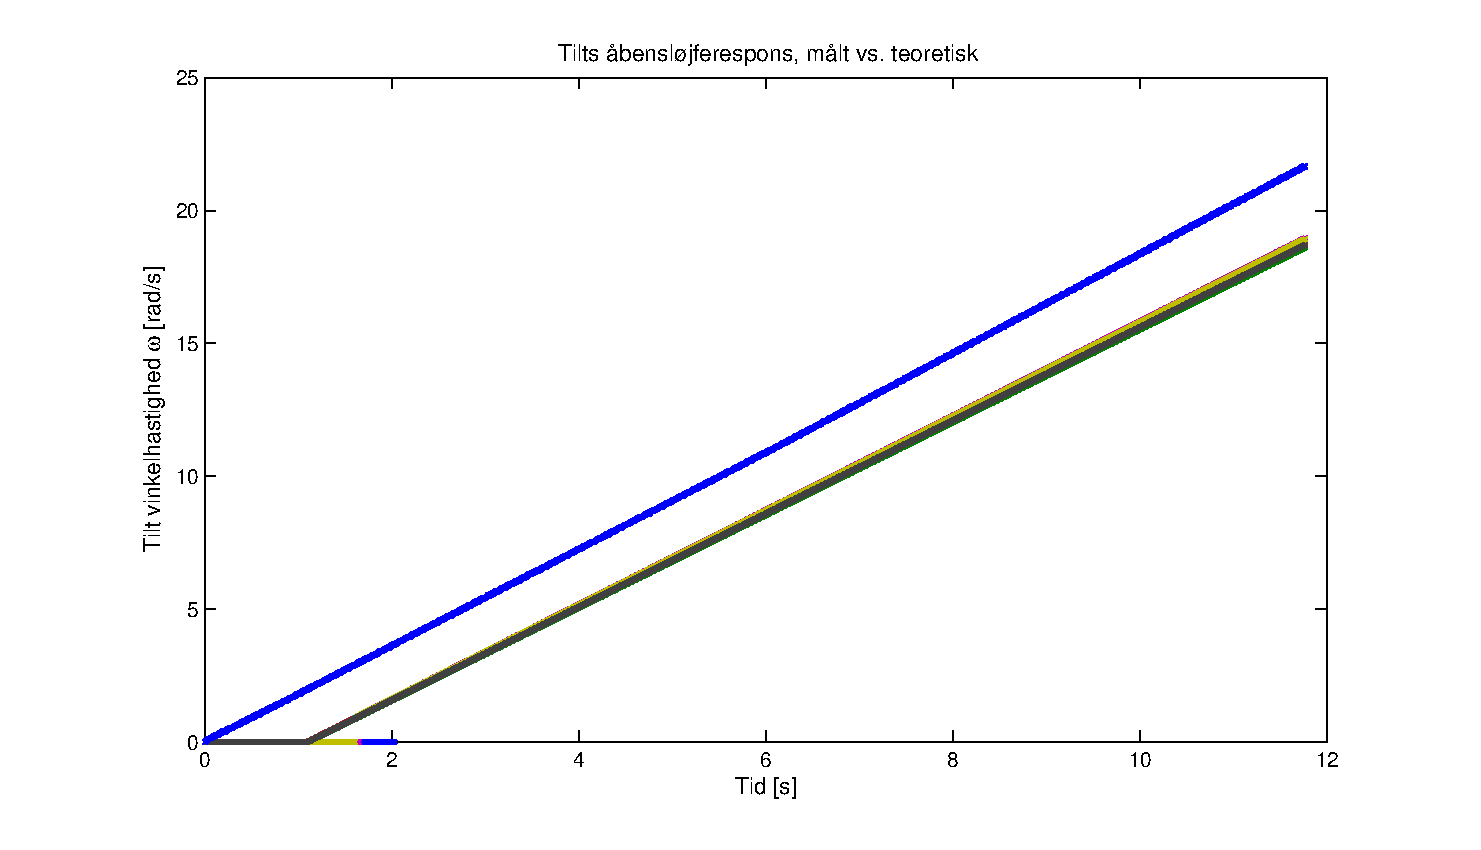
\includegraphics[width=0.7\textwidth]{./graphics/openloopVelocity1.eps}
	\captionsetup{width=0.7\textwidth}
	\caption[Tilt åbensløjferespons, målt vs. teoretisk]
		{Tilt åbensløjferespons, målt vs. teoretisk.
		Den teoretiske respons for de syv rampe-inputs er markeret med blåt.
		De andre kurver viser de målte responser.}
	\label{fig:openloopV1}
\end{figure}

Figur \ref{fig:openloopV1} viser den målte samt teoretiske vinkelhastighed,
som forudsagt af overføringsfunktionen \(s\cdot{}G_{tilt}\).
Det ses på figur \ref{fig:openloopV1}, at den største afvigelse er en tidsforsinkelse.
Dette skyldes, at lave spændinger ikke kan bevæge systemet.
Dødzonen af PWM-duty cycles, der ikke kan accelerere tilt-systemet er målt til at befinde sig inden for 14,65\% og for pan-systemet til 11,72\%.
Udover forsinkelsen fra dødzonen kan man på figur \ref{fig:openloopV1} aflæse
at den målte vinkelacceleration (hældningen af grafen) er marginalt mindre end den teoretiske.

Ønskes en mere nøjagtig matematisk model af PTS
er det altså en mulighed at indsætte dødzonen og evt. den ekstra dæmpning i modellen.
Det vælges dog at benytte de lineære åbensløjfeoverføringsfunktioner \(G_{pan}\) og \(G_{tilt}\)
som udgangspunkt for analysen der hører til regulatordesignet,
og i simuleringer af systemet at indsætte de tilnærmede værdier for dødzonen.

\subsection{Koordinattransformation}
\label{sec:koordinattransformation}
De kartesiske koordinater \(P_c=\left[x, y, z\right]\) skal transformeres til sfæriske koordinater
\(P_s=\left[\rho \text{ ; } \phi \text{ ; } \theta\right]\), hvor \(\phi\) og \(\theta\) er vinklerne for hhv. tilt og pan, og \(\rho\) er afstanden fra PTS til lerduen.
Til trackingen er kun \(\phi\) og \(\theta\) nødvendige.
Positionbestemmelsen som funktion af tiden for det kartesiske koordinatsæt beskrives i appendix \ref{subsubsec:para}.
Idet vinklerne skal bestemmes i forhold til PTS's rotationscenter og ikke koordinatsystemets origo,
skal PTS's rotationscenter PTS trækkes fra:
\(PTS=[\text{19,2 ; 0 ; 0,45}]\). 

\textbf{Flytning af origo}\\
% Koordinattransformationen tager udgangspunkt i den kartesiske stedvektor \(Pos\left(t\right) \), ligning \ref{eq:ks:vektorparabel3d} samt PTS's offset.
Origo flyttes, så kasteparablen kan beskrives ved vektor \(P_c\left(t\right)\), ligning \ref{eq:pf:stedvektorparabel}.
\begin{align}
\begin{split}
{ P }_{ c }\left(t\right)=Pos\left( t \right) -PTS = \left( \begin{matrix} - 9,34\cdot t-13,7 \\32,851\cdot t-19,3
\\-{ 4,91\cdot t }^{ 2 }+5,473\cdot t+2,6\end{matrix} \right) [\text{m}]
\label{eq:pf:stedvektorparabel}
\end{split}
\end{align}

\textbf{Koordinattransformation}\\
Sammenhængen mellem de kartesiske og de sfæriske koordinater kan ses på figur \ref{fig:thetaphi_degree}. 
Med PTS's offset er origo for det sfæriske koordinatsystem PTS's rotationscenter (skæringspunktet mellem de to rotationsakser).

\begin{figure}[!th]
\centering
\begin{tikzpicture}[scale=4]
\include*{./graphics/3d_in_xyz_plane}
\end{tikzpicture}
\caption[Sfærisk koordinatsystem til koordinattransformation]{Viser lerduens placering i det sfæriske rum som funktion af  \(\phi\), \(\theta\) og \(\rho\).}
\label{fig:thetaphi_degree}
\end{figure}

Som det fremgår af problemformuleringen modtager mikrocontrolleren lerduens
position som kartetiske koordinationer.
Transformationen fra kartesiske koordinater til
sfæriske koordinater gøres ud fra ligning \ref{eq:sv_koordi} nedenfor.
\begin{align}
{ P }_{ s }=\left( \begin{matrix} \phi  \\ \theta  \end{matrix} \right) =\left( \begin{matrix} { tan }^{ -1 }\left( \frac { { P }_{ c_{ z } } }{ \sqrt { { { P }_{ c_{ x } } }^{ 2 }+{ { P }_{ c_{ y } } }^{ 2 } }  }  \right)  \\ { tan }^{ -1 }\left( \frac { { P }_{ c_{ y } } }{ { P }_{ c_{ x } } }  \right)  \end{matrix} \right) 
\label{eq:sv_koordi}
\end{align}
hvor \(\phi\) og \(\theta\) er angivet i grader \citep[Kap. 10.6]{adam}.
